\documentclass[10pt, conference, compsocconf]{IEEEtran}

\ifCLASSINFOpdf
  \usepackage[pdftex]{graphicx}
  \DeclareGraphicsExtensions{.pdf,.jpeg,.jpg,.png,.pdf}
\else
  \usepackage[dvips]{graphicx}
  \DeclareGraphicsExtensions{.eps}
\fi

\graphicspath{{./images/}}

\usepackage{amsmath}
\usepackage{amsfonts}
\usepackage{amssymb}
\usepackage{setspace}
\usepackage{graphicx}
\usepackage{epsfig}
\usepackage{booktabs}

\hyphenation{op-tical net-works semi-conduc-tor}

\begin{document}

\title{Usage Management Overlay Architectures: Paths from Cross Domain Solutions}

\author{\IEEEauthorblockN{Christopher C. Lamb}
\IEEEauthorblockA{Department of Electrical and Computer Engineering\\
University of New Mexico\\
Albuquerque, NM, USA\\
cclamb@ece.unm.edu}
\and
\IEEEauthorblockN{Gregory L. Heileman}
\IEEEauthorblockA{Department of Electrical and Computer Engineering\\
University of New Mexico\\
Albuquerque, NM, USA\\
heileman@ece.unm.edu}
}

\maketitle


\begin{abstract}
Herein, we contrast filter-centric diode and policy-centric overlay approaches toward usage management of sensitive content from the perspective of cross-domain solutions and then demonstrate a path from current systems to distributed policy-centric overlay methods.  We first cover the need for overlay networks supporting usage management by highlighting the pending migration to utility computing models and the current shortcomings of those kinds of systems from a variety of perspectives.  We also briefly cover the state of usage management within these kinds of systems, also examining the known state of the art in proposed cross domain solutions.  The then compare and contrast the advantages of policy-based overlay systems to solving usage management issues over sensitive material and demonstrate a migration path from current to future solutions.  We close with our current and future directions of research. 
\end{abstract}

\begin{IEEEkeywords}
usage management; overlay networks; quantitative architecture evaluation;

\end{IEEEkeywords}

\IEEEpeerreviewmaketitle

Current enterprise computing systems are facing a troubling future.  As things stand today, they are too expensive, unreliable, and information dissemination procedures are just too slow.  Current approaches to partitioning information in cross-domain scenarios are simply unable to migrate to cloud environments because of reliance on control of physical hardware to enforce information separation.  The current approach of controlling information by controlling the underlying physical network, the traditional approach to securing information, does not scale into shared datacenters ~\cite{RedBook}.  This leaves large government and commercial organizations concerned with avoiding the exposure of sensitive data in a very uncomfortable position, where they cannot continue doing what they have done, and cannot migrate to what everyone else is doing.

Generally, systems handling sensitive information still do not use current commercial resources as well as they could and use costly data partitioning schemes.  Most of these kinds of systems are managed in house by the enterprise itself rather than exploiting lower cost cloud-enabled services.  Furthermore, many of these systems have large maintenance loads imposed on them as a result of internal infrastructural requirements like data and database management or systems administration.  In many cases networks containing sensitive data are separated from other internal networks to enhance data security at the expense of productivity, leading to decreased working efficiencies and increased costs.

These kinds of large distributed systems suffer from a lack of stability and reliability as a direct result of their inflated provisioning and support costs.  Simply put, the large cost and effort burden of these systems precludes the ability to implement the appropriate redundancy and fault tolerance in any but the absolutely most critical systems ~\cite{Tallon:2010:UDI:1735223.1735253}.  Justifying the costs associated with standard reliability practices like diverse entry or geographically separated hot spares is more and more difficult to do unless forced by draconian legal policy or similarly dire business conditions.

Finally, the length of time between when a sensitive document or other type of data artifact is requested and when it can be delivered to a requester with acceptable need to view that artifact is prohibitively long.  These kinds of sensitive artifacts, usually maintained on partitioned networks or systems, require large amounts of review by specially trained reviewers prior to release to data requesters.  In cases where acquisition of this data is under hard time constraints like sudden market shifts or other unexpected conditional changes this long review time can result in consequences ranging from financial losses to loss of life.

Federal, military, and healthcare computer systems are prime examples of these kinds of problematic distributed systems, and demonstrate the difficulty inherent in implementing new technical solutions.  They, like other similar systems, need to be re-imagined to take advantage of radical market shifts in computational provisioning.  New approaches to networking and information management present possible solutions to these kinds of problems by providing distributed information-centric approaches to data management and transfer ~\cite{proposal:info-sharing-strategy}.

Current policy-centric systems are being forced to move to cloud environments and incorporate much more open systems.  Some of these environments will be private or hybrid cloud systems, where private clouds are infrastructure that is completely run and operated by a single organization for use and provisioning and hybrid clouds are combinations of private and public cloud systems.  Driven by both cost savings and efficiency requirements, this migration will result in a loss of direct control of computing resources by involved organizations as they attempt to exploit economies of scale and utility computing.

Robust usage management will become an even more important issue in these environments.  Federal organizations poised to benefit from this migration include agencies like the United States National Security Agency (NSA) and the United States Department of Defense (DoD), both of whom have large installed bases of compartmentalized and classified data.  The DoD realizes the scope of this effort, understanding that such technical change must incorporate effectively sharing needed data with other federal agencies, foreign governments, and international organizations ~\cite{proposal:info-sharing-strategy}.  Likewise, the NSA is focused on using cloud-centric systems to facilitate information dissemination and sharing ~\cite{proposal:nsa-cloud}.

Cloud systems certainly exhibit economic incentives for use, providing cost savings and flexibility, but they also have distinct disadvantages as well ~\cite{proposal:privacy-security-trust-cloud}.  How to address these issues is an open research question.  Organizations ranging from cloud service providers to the military are exploring how to engineer solutions to these problems, and to more clearly understand the trade-offs required between selected system architectures ~\cite{proposal:assured-info-sharing}.  The problems themselves are wide ranging, appearing in a variety of different systems.  Military and other government systems are clearly impacted by these kinds of trust and security issues, and they also have clear information sensitivity problems.  This, coupled with the fact that these organizations have been dealing with these issues in one form or another for decades make them very well suited for prototypical implementation and study.

This chapter will cover national and international standards in this area, current solutions in place to address some of these problems, the state of the art in information networks, and other related work.  Organizations have been trying to standardize security approaches since the 1980's, starting with the notorious Orange Book ~\cite{OrangeBook}, and ending with today's NIST cloud standards ~\cite{NIST800:144}.  Information-centric networks are a new approach to information management that promises more efficient content  management and supplies new capabilities for information security. The DoD has been key in some of these efforts, and continues to play such a role today, demonstrated in the state of the art in today's cross-platform solutions.  The second chapter introduces and analyzes a proposed architectural taxonomy to address the information sharing goals held by the DoD through the Unified Cross Domain Management Office (UCDMO), and the third describes in detail the development of this prototypical system, starting with a single-system proof-of-concept and working through the current nation-spanning cloud network.  The final chapter covers specific experimental results and analysis of these techniques from a confidentiality, integrity, and availability perspective.

\subsubsection*{Shortcomings of Current Systems}
Having reviewed the current state of the art of these kinds of cross domain solutions,  they still have clear similarities, and in fact have not progressed far beyond the initial notions of how these kinds of systems should work.  They still, for example, all use some kind of filter chaining mechanism to evaluate whether a given data item can be moved from a classified to an unclassified network.  Both NSA models used filters explicitly, as did the BAH model.  They all use a single guard as well, a sole point of security and enforcement, providing perimeter data security, but nothing else.  In each of these current system architectures, users are only allowed to exchange one type of information per domain.  The physical instantiations of these models are locked by operational policy to a single classification level limit.  Users cannot, for example, have Top Secret material on a network accredited for Secret material.  Finally, these models violate the end-to-end principle in large service network design, centralizing intelligence rather than pushing that intelligence down to the ends of the system \cite{Blumenthal:2001:RDI:383034.383037}.

\subsubsection*{Characteristics of Future Systems}
Future systems will generally demonstrate decentralized policy management capabilities, infrastructural reuse, the ability to integrate with cloud systems, and security in depth.  Policy management is decentralized and integrated within the fabric of the system.  The system is both more secure and resilient as a result, better able to control information and operate under stressful conditions.  Multi-tenancy can lower costs and increase reliability and is furthermore a common attribute of cloud systems.  An appropriately secured system facilitates integration of computing resources into multi-tenant environments.  The ability to handle multi-tenant environments and to reliably secure both data at rest and data in motion leads to computational environments deployable in cloud systems.  Finally, systems must operate under \textit{all} conditions, including when they are under attack or compromise \cite{proposal:ron-ross}.  Ergo, they must provide protection to sensitive data in depth.

\subsection{Other Related Work}
This work introduces the notion of usage management embedded in a delivery network itself.  It also provides an in-depth analysis of the challenges and principles involved in the design of an open, inter-operable usage management framework that operates over this kind of environment. Besides referencing the material we have covered in depth to portray the current state of the art, the analysis includes application of well-known principles of system design and standards~\cite{BlCl:01,Cl:88,ClWrSoBr:02}, research developments in the areas of usage control~\cite{PaSa:04,JaHeLa:10}, policy languages design principles~\cite{JaHeMa:06}, digital rights management (DRM) systems~\cite{JaHe:09},  and interoperability~\cite{JaHe:04,HeJa:05,KoLaMaMi:04,coral,marlin} towards the development of supporting frameworks.

While a large body of work exists on how overlay networks can use policies for \textit{network} management, very little work has been done on using usage policies for \textit{content} management.  The primary contribution in this area focuses on dividing a given system into specific \textit{security domains} which are governed by individual policies \cite{4457175}.  This system fits into our proposed taxonomy as an $\alpha$-type system as it has domains with single separating guards.

A large body of work currently exists with respect to security in and securing overlay networks.  These kinds of techniques and this area of study is vital to the production development and delivery of overlay systems, but is outside the scope of this work.

\subsection{Cross Domain Solutions}
The Unified Cross Domain Management Office (UCDMO) supports efforts do develop other specific solutions that have been presented over the past few years within the government space to handle this kind of information management.  The National Security Agency set the standard in this area initially.  In 2009, at a conference sponsored by the UCDMO, Booz $\mid$ Allen $\mid$ Hamilton and Raytheon presented alternative notional architectures contrasting with current NSA-influenced approaches \cite{proposal:nsa-arch,proposal:gig-arch,proposal:bah-arch,proposal:raytheon-arch}.

\section{Taxonomies of Usage Management Overlay}
A clear taxonomic organization of potential steps in approaching finer grained policy based usage management helps in describing the difficulties inherent in developing potential solutions as well as aiding in planning system evolution over time. Here, we have five distinct types of integrated policy-centric usage management systems, as shown in Table \ref{table:model:taxonomy}.  Of these five, only the first two levels are represented in current system model.

\begin{table*}[tp] %
\centering %
\begin{tabular}{clcc}
\toprule %
$ Name$ 	& $Description$ \\\toprule %
$\phi$ 		& The initial level of this taxonomy, $\phi$ classified systems \\
 			& have a single guard without policy-based control \\\midrule
$\alpha$	& $\alpha$ classified systems have a single guard by have begun \\
			& to integrate policy-based control \\\midrule
$\beta$		& Systems that have begun to integrate policy-based control with \\
			& router elements are in the $\beta$ category \\\midrule
$\gamma$	& Systems that have integrated policy-based control with routing \\
			& and computational elements \\\midrule
$\delta$	& Continuous policy-based control with \textit{smart licensed} artifacts \\\bottomrule
\end{tabular}
\caption{Proposed Usage Management Taxonomy}
\label{table:model:taxonomy}
\end{table*}

In this taxonomy, it is not required that systems pass through lower levels to reach higher ones.  This taxonomy represents a continuum of integration of usage management controls.  Systems can very well be designed to fit into higher taxonomic categories without addressing lower categories.  That said however, many of the supporting infrastructural services, like identification management or logging and tracing systems, are common between multiple levels.

The taxonomy itself starts with the current state, integrating policy evaluation systems into the network fabric gradually, moving away from filters, then by adding policy evaluation into the routing fabric, then the computational nodes, and finally by incorporating evaluation directly into content.

\subsection{$\phi$-level Overlay Systems}
The $\phi$ classification consists of systems like the initial NSA and BAH notional models.  These systems consist of two distinct domains, separated by a filter-centric single guard.  The initial NSA system model is clearly of this type, separating two domains with a guard using filter chains.  The BAH model is also of this type, using a Filter Segment to evaluate data packages transmitted between interface segments attached to specific domains.

\begin{figure}[!t]
\centering
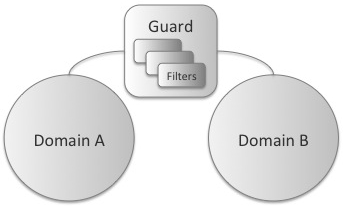
\includegraphics[width=3in]{model-phi-crop}
\caption{Taxonomy ($\phi$)}
\label{fig:model:taxonomy-phi}
\end{figure}

Generally one of the domains supports more sensitive information than the other, but that is not always the case.  In the models we have examined this has certainly been true, but classified information for example  is commonly stored in \textit{compartments} which are separated by clear \textit{need-to-know} policies enforced by access lists and classification guides.  These kinds of compartments contain information at similar levels of classification, but contain distinct informational elements that should not be combined.

In these kinds of systems, specific rules regarding information transfer and domain characterization are tightly bound to individual filter implementations.  They are based on \textit{a priori} knowledge of the domains the guard connects, and therefore are tightly coupled to the domains they connect.  Furthermore, the filter elements are standalone within the system, in this classification, not availing themselves of external resources.  Rather, they examining information transiting through the filter based purely on the content of that information.

\subsection{$\alpha$-level Overlay Systems}
The $\alpha$ overlay classification contains systems that have begun to integrate policy-centric usage management.

Both policies and contexts are dynamically delivered to the system.

The dynamic delivery of context and policies allows these kinds of systems more flexibility with policy evaluation.

The $\alpha$ category begins to integrate policy-centric management rather than using strict content filtering.

\begin{figure}[!t]
\centering
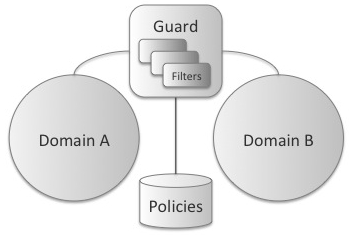
\includegraphics[width=3in]{model-alpha-crop}
\caption{Taxonomy ($\alpha$)}
\label{fig:model:taxonomy-alpha}
\end{figure}

Here, we again have at least two domains, Domain A and Domain B, though we could potentially have more.  $\phi$ type systems require domain specific information to be tightly coupled to the filter implementations.  Separating the permissions, obligations, and other constraints from the filters and incorporating them into a specific separate policy entity frees the Guard from this coupling and provides additional flexibility to the system.

The guard can continue to use filters to process data.  These filters however are now more generic and decoupled from the specific domains it manages.  The choice of using a specific filtering model rather than some other kind of construct is a design detail level to implementers.  That said however, individual filters will be remarkably different and still need to understand the ontologies over which specific licenses are defined.

The policy repository is key to the implementation and differentiation of this taxonomy category.  This repository can be implemented as a separate repository keyed into via a data artifact's unique URI, for example.  It could also represent a policy sent in tandem with a data artifact in a data package.

The policy repository may be implemented as some kind of external service, and as such, represents the first such external service explicitly used in this taxonomy.  Other external services may well exist and be used to adjudicate information transfer decisions as well.

\subsection{$\beta$-level Overlay Systems}
The $\beta$ taxonomic category begins to integrate policy-centric processing with router elements in a given network.  While this work is centered on using overlay technology to illustrate and implement these concepts, it is important to note that this kind of distributed policy-centric processing could very well be distributed into the physical routing fabric of a given network as well by extending Software Defined Networking systems like OpenFlow \cite{proposal:openflow}.

\begin{figure}[!t]
\centering
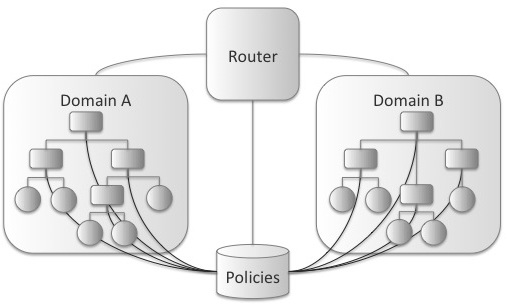
\includegraphics[width=3in]{model-beta-crop}
\caption{Taxonomy ($\beta$)}
\label{fig:model:taxonomy-beta}
\end{figure}

In this model we can also host multiple domains as a result of flexible policy-based content examination.  Each domain hosts a network of some kind, though that hosted network could very well be a degenerate network of a single system.  Each network hosted in a domain is hierarchical, with specific computational nodes embodied by workstations, tablet computers or mobile devices, and routing points embodied by routers or switches of some kind.

Policy evaluation in this model has begun to penetrate into the routing elements of the specific domain networks.  Here, note that we have started to penetrate into the routing fabric of the network by doing content evaluation at router points.  Content-based switching networks have been successful in other domains, and such techniques can be used here to provide policy evaluation capabilities.  

Certain types of traffic are easier to evaluate than others however.  For example, HTTP requests and responses are easier to examine that TCP packets.  When examining TCP packets, systems generally require additional context to select an appropriate packet window (e.g. the number of packets cached for examination).  HTTP traffic does not usually require this kind of flexibility.

This migration of policy evaluation into the routing fabric provides for enhanced data security and better network management, especially if part of a network is compromised.  Now that policy decisions can be made at the router level in a given network, we are starting to have network security in depth rather than simple perimeter protection.  This not only provides the ability for additional information protection, but also allows for different compartments holding information at different need-to-know levels to be created ad-hoc under different routing segments.  In cases of network compromise, this kind of dynamic policy enforcement can also allow for quick node excision as well.

\subsection{$\gamma$-level Overlay Systems}
The $\gamma$ compartment has integrated policy evaluation with compute and routing nodes.  Here, policies can be evaluated against content at all network levels --- nodes emitting requests, nodes fielding requests, and all routing elements in between.

\begin{figure}[!t]
\centering
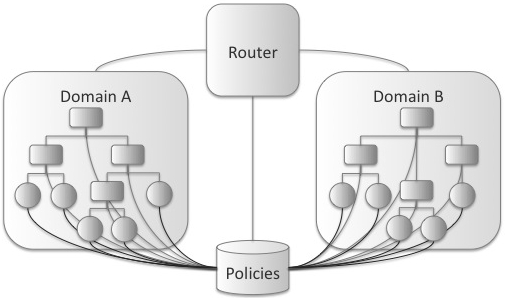
\includegraphics[width=3in]{model-gamma-crop}
\caption{Taxonomy ($\gamma$)}
\label{fig:model:taxonomy-gamma}
\end{figure}

We see that the policy repository is supplying services to all computational elements in both domains.  This gives us increased granularity with respect to data compartmentalization by integrating information security into each network element.  At this point, the network can create compartments of single nodes, while previously in $\beta$ level systems compartments could only be created under specific routing elements.  At this level, we can also provide services revoking data access based on policy evaluation decisions when needed.

Furthermore, individual node exclusion is possible as well. $\beta$ classified systems could excise network elements under specific routers by dynamic policy application.  Now, we can apply the same functionality to individual compute nodes.  For example, if a networked device like a smart phone is compromised, that device can be removed from access quickly or used to feed mis-information to adversaries.

\section{Taxonomic Analysis}
The various levels of the taxonomy vary primarily with respect to the inclusion of policy-based usage management and overlay structure.  $\phi$ type systems are not structured with overlay use in mind, nor do they use policy-centric management.  Conversely, $\gamma$ type systems are both purely policy oriented and completely overlay structured.

As systems move through the various levels of the taxonomy they gradually move from one side of the spectrum to another.  Overlay structures, hierarchical or otherwise, gradually migrate into the network begining with $\beta$ systems.  Policy orientation is injected into the architectures starting with $\alpha$ systems and moving into the network fabric in parallel with overlay inclusion.

\subsection{Policy-centricity}
In these systems policy based management supplies distinct advantages over filter-centric information control.  This kind of policy-centric usage management is more content specific than filters, more flexible, and is more expressive than filter-centric systems.

\subsubsection*{Content Specific}
Filters, in filter-based systems, are not coupled to the content passing through the system.  Rather, they are usually tied to the characteristics of attached networks.  For some filters, that is not problematic.  Malware filters, for example, are very general and do not need to have an understanding of filtered content and are not sensitive to that content at all, though they can be very sensitive to specific context.  This limitation does however prohibit filters from doing anything content specific.  Due to their deployment limitations, in that they are deployed to such a system via a process distinct from processing content, they are unable to use presented content or current dynamic context to influence information processing decisions.

Consider content $c$ impacted by a dynamic context $d$ where $d$ is defined in terms of the content itself, the person or system requesting that content, and the environment in which that request is made.  Here, only under certain specific environmental conditions is that requesting agent allowed access to the requested content.  Ergo, the decision with regard to pass the content to the requester is based upon characteristics of the content related to dynamic changes within the environment.  A filter-centric solution like that contained within the $\phi$ level of the taxonomy is unable to change filter rules based on changes like new content or environmental alteration.  A policy-based system, on the other hand, is able to express the content specific policy easily for more dynamic evaluation.

For example, if $c$ contains information that can only be accessed for a specific time period, a static filter simply cannot determine that the information in $c$ is no longer appropriate for dissemination after that time period ends.  That kind of evaluation requires meta-data associated with $c$ that specifically describes these time bounds and a dynamic contextual evaluator able to determine when that window of access has closed.  That meta-data in this case is a policy.

\subsubsection*{Flexibility}
Policy-centric systems are more flexible than filter-based counterparts.  In a filter-based solution, the type of content that can be evaluated is tightly coupled to the filters installed.  If a given piece of content is new to a given filter-centric solution, that content cannot be appropriately examined and must be submitted for human review.  A policy-based system is designed to be more general.  Based upon a common ontology ~\cite{JaHeLa:10}, the evaluation system can be very general with respect to it's evaluation of a given policy.  A general policy engine can handle a great variety of different content as long as the policies associated with that content correspond to known domain ontologies.  This generality leads to a greater amount of flexibility with respect to what can be expressed in a specific policy, and leads to a more flexible maintainable system.

A filter is going to have a specific responsibility, like redacting sensitive words from a document, for instance.  In order for that filter to redact those sensitive words, it must have access to some kind of list of what those sensitive words are.  Remember, $\phi$ level systems use static filters, so that filter can only be updated when the filter itself is updated.  Now a policy-centric system on the other hand can have a policy associating sensitivity with various areas of content in a specific document.  In this case, all the system must do is understand the sensitivity described in the policy associated with the content, and can then redact that content if needed.  The ontology describing the areas of sensitivity will change more slowly that the possible content itself, leading to a more flexible maintainable system.

This is of course a simple example solvable by creating a dynamic list; the key point of the above example is that the specificity of the filters requires additional complexity in the filter system itself.  The generality of the policy-centric system allows the complexity to be more clearly expressed and contained within the policy file.

\subsubsection*{Expressiveness}
While filters can process content at specific perimeter points, it's lack of reach into a given network fabric limits the power a given filter can actually have over transmitted content.  A policy associated with content, when transmitted with content, can reference much more than the semantics of the protected content.  That policy can describe specifically, in detail, how that content can be used.  Filters simply cannot exercise that level of control.

Assume a distributed system with multiple filter points.  In this kind of system, information distribution can be controlled via deployed filters at a relatively fine level of granularity.  This kind of distribution control cannot influence the use of protected content however --- one that content is distributed, possessors are accorded full access.

Policy enabled systems are not limited in this way.  Policies, when coupled with policy evaluation tools, can exercise control not only over distribution and routing, but also over use of distributed content at endpoints.

These advantages accrue in usage management systems as policy capabilities are propagated through the overlay fabric.  Some of these advantages, like expressiveness, appear simply by beginning to use policies instead of filters.  The remaining two have more of an impact as additional policy-centric nodes combine to form an overlay system suitable for cloud deployment increasing their impact as they move from $\alpha$ to $\delta$ types of systems.

\subsection{Overlay Structure}
Overlay structure integration exhibits clear advantages over single point perimeter systems as well.  Specifically, overlay systems are more partition-able than perimeter solutions, enable content throttling, provide capabilities for dynamic content control, and allow content to be more traceable.

\subsubsection*{Partition-ability}
Administrators typically deploy filter-based perimeter protection at strategic routing points on secure networks.  These kinds of networks are designed with specific regions of enhanced sensitivity separated by cross domain management systems regulating information flows \cite{proposal:nsa-arch,proposal:raytheon-arch,proposal:bah-arch}.  While sensible from the perspective of each protected region as a secure domain, this design thinking begins to fall apart when exposed to the very real threat of the malicious insider.  Boundary-centric information flow control is impossible to realistically achieve when the actual boundaries between malicious actors and system users is constantly in flux.  When a malicious actor can be anywhere within a system, boundaries are simply too dynamic to be realistically recognized.  In order to surmount this fluid system posture, designers must adopt a security in depth mindset.

Application layer overlay networks enable this kind of defense in depth via the possibility of partitioning.  A given overlay system depending on the level of overlay inclusion can partition the user space and by doing so decrease the attack surface available to a malicious insider.  $\phi$ and $\alpha$ level systems based on perimeter filters simply do not present this ability.  Systems beginning with $\beta$ provide the potential to create need-to-know cells of finer granularity up to $\delta$ type systems in which cells can be created at the level of specific content.  These need-to-know cells serve to help quarantine possible intrusion into the sensitive distribution fabric if that fabric is compromised by helping isolate that system failure within the compromised cell.

For example, assume a hypothetical system with nine nodes connected along a single data plane within an prototypical secure network.  With perimeter defenses, if one of those nodes is compromised, a malicious actor can begin to monitor communications traffic between all network nodes, effectively compromising the entire network.  In this same network, if designers partition the system into three overlay cells of three nodes, a similar intrusion in one of those cells will effectively only compromise that cell, leaving the other two cells unaffected.  This decrease in possible targets for compromise effectively decreased the network attack surface from any give node by $\frac{2}{3}$, correspondingly increasing the security posture of the system.

\subsubsection*{Content Throttling}
Perimeter located filter systems only have the opportunity to control sensitive traffic at that initial boundary.  Information located in repositories behind that boundary is not subject to control if it is retrieved by an agent also ensconced behind that same system boundary.  Granted, control can be exerted at the repository level, but in a system with more than one repository, this is if limited impact.

A partitioned cell-oriented system, on the other hand, provides greater opportunity for information monitoring and control.  The partitions applied atop the physical infrastructure provides additional potential control points requests must cross in order to access needed information.  Furthermore, less random cell design provides the capability to unify repositories however needed to provide tight control of information dissemination.

Our hypothetical nine-node system, for example, provides no control over information dispatched from one of the contained nodes to other contained nodes in its initial design form.  There are simply no control points within that nine-node network at which to monitor and control information flow.  Partitioning that space into three three-node cells provides at least two potential control points for inter-cell requests at which information flow can be monitored.  In cases where a malicious insider is actively collecting and hoarding data for exfiltration, these additional control points give system administrators the ability to automatically throttle the rate at which sensitive material can be accessed by users to increase the cost of data collection and increase the likelihood of agent discovery.

\subsubsection*{Dynamic Content Control}
Singular perimeter solutions due to their lack of internal control points also forgo the ability to provide dynamic content control.  Once information has traversed a given perimeter access point, it is no longer under the control of that point and can no longer be retrieved, accessed, monitored, or modified.  Overlay solutions with internal control points can provide the ability to continually monitor and control disseminated information.

Within a given overlay system, depending on that system structure, data can be more rigorously controlled.  $\beta$ and $\gamma$ systems provide the ability to dynamically change information access via contextual changes at a finer grained level than perimeter solutions can.  $\gamma$ systems can in fact provide the ability to retract information access on a per request basis.

This kind of control is especially useful in situations where external partners may temporarily need access to sensitive information for a specific short period of time, say during some kind of joint exercise or activity.  $\gamma$ systems can provide that access only during the window of operation, and retract that access when that window closes.  This kind of use is common in joint military operations with coalition partners, for example.

\subsubsection*{Traceability}
The singular location of perimeter filter solutions also precludes easy information traceability.  Data requests within a given network sans internal controls is more difficult to trace than an overlay solution with a partitioned cell structure that is tailored to the specific information requested (say, XML databases or semantic web content).  The partitioned overlay requires requests to traverse multiple routing nodes at which request and response content can be examined and stored for later analysis and visualization.  Perimeter solutions without this kind of structure simply cannot monitor flows at this finer-grained level.

The strengths of overlay systems over single perimeter points gradually increase as overlay structures increasingly permeate any given system.  Some abilities, like access repudiation, can only occur with smart licensed artifacts at the $\gamma$ level.  Others, like traceability or throttling, become more effective as a system architecture traverses from lower to higher levels of capability within the proposed taxonomy.

\section{Conclusion}
The conclusion goes here. this is more of the conclusion

\bibliographystyle{IEEEtranBST/IEEEtran}
\bibliography{bib/proposal,bib/drm}

\end{document}


